\documentclass[12pt,titlepage]{ltjsarticle}
\usepackage[top=25truemm,bottom=25truemm,left=20truemm,right=20truemm]{geometry}
\usepackage{luatexja-fontspec}
\usepackage[ipaex]{luatexja-preset}
\usepackage{amsmath}
\usepackage{empheq}
\usepackage{color}

\usepackage{lastpage}
\usepackage{fancyhdr}
\pagestyle{fancy}
\lhead{}
\rhead{E1333  廣氏 宣勇}
\cfoot{\thepage/\pageref{LastPage}}%フッタ中央に"今のページ数/総ページ数"を設定
\renewcommand{\headrulewidth}{0.0pt}%ヘッダの線を消す


\title{\huge 電気情報工学概論 調査事項報告書}
\author{E1333  廣氏 宣勇}
\begin{document}
\date{2015年6月22日}
\maketitle
\section{キャパシタの種類と構造について}

主要なキャパシタの特性について表\ref{tab:r1}に示す。
\begin{figure}[htbp]
    \centering
        \renewcommand{\figurename}{表}
        \caption{主要なキャパシタの特性}
        \label{tab:r1}
        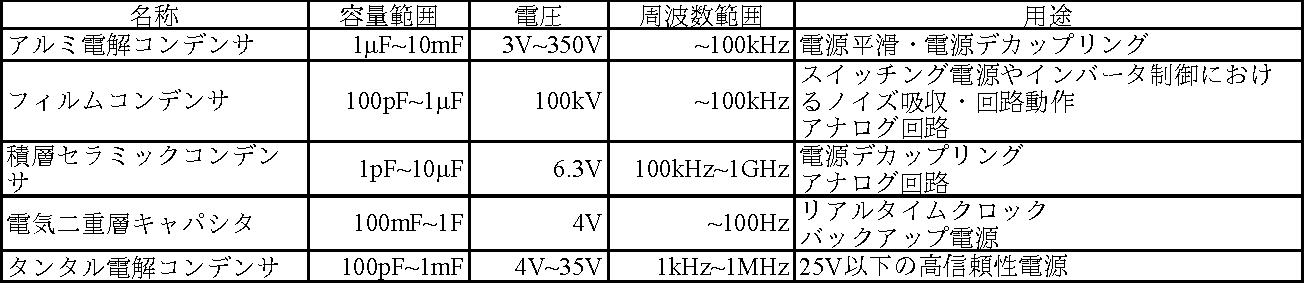
\includegraphics[width=\linewidth]{resc1.pdf}
\end{figure}

それぞれの構造は以下のとおりである。
\begin{itemize}
\item アルミ電解コンデンサ  :陰極にアルミ箔、陽極に酸化皮膜付きのアルミ箔、その間に電解紙と電解液が入っている。
\item フィルムコンデンサ   :金属箔にプラスチックフィルムを重ねて、それを巻き取って作る。
\item 積層セラミックコンデンサ:それぞれの極板から電極が交互に生え、層をなしている。
\item 電気二重層キャパシタ  :「集電電極と活性炭の電極を重ねたもの」1対と電解液から成る。
\item タンタル電解コンデンサ :陰極に銀、陽極に酸化皮膜付きのタンタル、その間に固体の二酸化マンガンとグラファイトが入っている。
\end{itemize}

\section{発電所の発電機の仕組みについて}

太陽光発電所について報告する。

太陽光発電所はメガソーラーとも呼ばれており、太陽光が再生可能エネルギーであることから、メガソーラーは最近注目を集めている。
メガソーラーは大きく分けて「太陽電池モジュール」、「パワーコンディショナ」、「連系変電設備」の3つの装置からなる。
\begin{itemize}
\item 太陽電池モジュール

太陽電池モジュールはシリコンなどの半導体でできており、半導体は光が当たると電子を放出する性質を持っている。
放出された電子の向きとは逆の方向に電流が生じ、これが電力となる。
太陽電池モジュール一つの発電量はそれほど多くないが、それを多数連結させた「アレイ」と呼ばれるものを大量に配置することで使用に堪える電力を生み出せる。

\item パワーコンディショナ

太陽電池モジュールが生み出す電流は、半導体に当たる光の量に比例する。
もし太陽電池モジュールから商用交流を取り出そうと思うなら、太陽光を高速(1秒間に50\verb|~|60回)で強弱させなければならない。
それは不可能なので、取り出した直流を交流に変換するのがパワーコンディショナの仕事である。

\item 連系変電設備

上記の2つの装置で発電は可能であるが、メガソーラーは発電所なので、電気を使うところに電力を配送しなければならない。
そのため、電力は電力会社の送配電線に送らないといけないのだが、その時に作った電力の電圧を調整する設備が連系変電設備である。
\end{itemize}

\section{発電所で用いられる変圧器について}

連系変電設備に使われる変圧器は最終的に生み出される電力に大きく関係する。
ここではメガソーラーで実際に使われる油入(OF式, Oil-Feeding)変圧器について報告する。

変圧器は「'ロ'の字型の薄いケイ素鋼の板を何枚か積み重ねて作る鉄心」と「巻き数の違う2つの巻線」から成る。
一方の巻線に交流電圧に電圧を印加すると、もう一方の巻線に変圧された電圧が発生する。
どれだけ変圧されるかは巻き数の比によって決まる。

この時巻線は発熱し、これは変圧器の劣化につながる。
巻線の熱を取るために変圧器の内部を絶縁油で満たした変圧器が油入変圧器である。

\section{電動機の可変速運転について}

DCモータとパルスモータの可変速運転について報告する。
\begin{enumerate}
\item DCモータ

DCモータの速度はDCモータのコイルに流れる電流に比例する。
電流を変化させる方法は電圧自体を下げる方法とPWM方式を用いて電圧のかかる時間を短くする方法がある。

\item パルスモータ

パルスモータの速度は単位時間あたりの入力パルス数に比例する。
入力パルス数を大きくするには電源の周波数を大きくすれば良い。

\end{enumerate}

\section{回生動作について}

モータに電流を流すと(この方向を順方向とする)、回転する。
モータが加速すると、モータに接続された負荷にはエネルギーが溜まる。
モータに流れる電流を小さくすると、モータは減速する。
この時、モータに接続された負荷に溜まったエネルギーは放出される。
放出されたエネルギーは逆方向にモータを通る電流を作り出す。
この電流のことを回生電流といい、この挙動を回生動作という。
このとき、モータは発電機になっていると見ることができる。
事実、ブレーキをかけることで発電する回生ブレーキは電気自動車などで使われている。

しかし、モータがインバータから電力を供給されている場合はこの回生動作がネックとなる。
インバータは交流を作るため、モータは必ず減速し、回生電流が必ず発生する。
インバータに大きな回生電流が逆流すると出力端子の電圧が上昇して過電圧状態となり、インバータの故障を引き起こす。
回生電流の大きさはモータの減速度に比例する。
そのため、回生電流を小さくするには、モータの減速度を小さくするために「インバータが電圧を下げる速度」を下げるか、
インバータの出力端子に抵抗を挿入し、出力端子の電圧上昇量を小さくするとよい。

\end{document}
